%\documentclass[draftcls,onecolumn,journal]{IEEEtran}
\documentclass[journal]{IEEEtran}
\usepackage{algo}
\usepackage{cite}
\usepackage{url}

\ifx\pdfoutput\undefined
\usepackage{graphicx}
\else
\usepackage[pdftex]{graphicx}
\fi

\makeatletter
\let\NAT@parse\undefined
\makeatother

\ifx\pdfoutput\undefined
\usepackage[hypertex]{hyperref}
\else
\usepackage[pdftex,hypertexnames=false]{hyperref}
\fi

\hyphenation{dy-namic em-bed-ding in-ter-na-tion-al con-fer-ence know-ledge}


\begin{document}
\title{
  Multilevel Circuit Partitioning with Maximal-matching Based
  Clustering and Signal-flow Based Clustering
} 
\author{Wai-Shing~Luk,~\IEEEmembership{Member,~IEEE}}%
% The paper headers
\markboth{Journal of \LaTeX\ Class Files,~Vol.~1, No.~11,~November~2002}{Shell \MakeLowercase{\textit{et al.}}: Bare Demo of IEEEtran.cls for Journals}
\maketitle

\begin{abstract}
Primal-dual algorithm is derived for solving
the maximal-matching based clustering (MMC) problem within the multilevel
circuit partitioning framework. Compared with the usual greedy approaches, the
method generates high-quality clusters using less amount of time. 
When signal direction information is available from input
circuit, a signal-flow clustering method is presented. An algorithm for
handling feedback paths and bi-directional pins is proposed.
Experiments show that the resulting methods produce a
very promising quality of cutsize and run-time performance compared
with the recent cutting--edge packages \verb+hMetis+ and \verb+UCLA_MLPart+. 
The tradeoffs between different implementations are also discussed.   
In particular, the tradeoff between reliability and performance is
investigated.
%that allowing illegal moves during the iterations often
%dramatically improve the performance, whereas such iterations will
%eventually lead to a legal solution is not guaranteed.
\end{abstract}

\begin{keywords}
Circuit partitioning, multilevel partitioning, clustering, 
multiway partitioning, hypergraph partitioning, primal-dual.
\end{keywords}

\IEEEpeerreviewmaketitle

\section{Introduction}
\PARstart{C}{ircuit} partitioning is a fundamental CAD problem and
finds application in diverse areas such as top-down placement and
circuit simulation. The problem is usually expressed in graph theoretic
term. Recall that a hypergraph $H$ is a pair of sets $(V,E)$. The set 
$V=\{v_1, \ldots, v_n\}$ is a set of the {\it vertices}  
and $E=\{e_1, \ldots, e_m\}$ is a set of {\it hyperedges} (or simply
{\it edge}). Each hyperedge $e_i = \{v_1, \ldots, v_k\}$ is a subset of
$V$. A {\it weighted hypergraph} is
a hypergraph with a function $w: V \mapsto \mathbf{R}$. To connect a
circuit (or a {\it netlist}) with the hypergraph notations, 
each {\it module} is represented by a
vertex in $H$. A module can be either a {\it cell} or a 
{\it pad}. The area of each module is represented by the weight
function of vertex $w(v_i)$. Each {\it net} is represented by a hyperedge. 
Consider the {\it Minimum Balanced Cut} problem that requires to
partition the vertices into $K$ disjoint subsets $V_1, \ldots, V_K$
such that each subset has equal sum of vertices weights.
The objective of the problem is to minimize the number
of hyperedges crossing the partition, which is called the {\it cutsize}.
The Minimum Balanced Cut problem is proved NP-complete.
Nevertheless, because of the importance of the problem,
extensive research on finding efficient heuristics have been studied 
(c.f. the survey paper of~\cite{survey_1995}). 
They include methods that are based on local search 
(e.g. the Kernighan--Lin (KL) method~\cite{KL_1970} 
and the Fiduccia--Mattheyses (FM) method~\cite{FM_1982}),  
methods are that based on simulated annealing
(e.g~\cite{simulated_evolution_1990}), 
methods that based on genetic algorithm 
(e.g.~\cite{adaptive_genetic_1999,genetic_1999}), 
methods are that based on tabu search 
(e.g.~\cite{tabu_1993}), 
methods are that based on neural network
(e.g.~\cite{hopfield_1994,neural_network_1995,neural_network_tcad_1990,stochastic_neural_network_1996},
methods that are based on mathematical programming 
(e.g.~\cite{gradient_FM_1995, eigenvector_1996}), 
methods that are based on multilevel paradigm (see below) 
and the hybrid of those methods (e.g.~\cite{hybrid_multilevel_genetic_1996}).

In circuit partitioning, currently the standard approach is the
iterative improvement method. Given an initial feasible
solution, in the classical local search approach, modules are
successively moved between partitions until there is no more positive
{\it gain} on the current solution. While the iterative improvement
method generates new solutions by performing sequences of moves on
the current solution per pass. As a result, even though a first few moves
may produce negative gain, if the final sequence of moves produces
positive gain, the algorithm can still proceed and hence generates
smaller cutsize in general. One of the best iterative
improvement algorithms is known as the 
Fiduccia--Mattheyses (FM) algorithm~\cite{FM_1982}.
In the FM algorithm, an array of {\it gain buckets} is used to
maintain the gains of moves. Since the maximum gain for a single
move is bounded by $[-p_{max}, p_{max}]$ where $p_{max}$ is the maximum
pin count of module, the algorithm runs in nearly linear
time per pass if $p_{max}$ is small. It makes the FM algorithm very
attractive as a basic algorithm. However, due to the natural of the
local search, the iterative improvement method can only find solutions
in local minimum.

%% May be able to delete
In the conventional graph partitioning problem, a method of using
eigenvectors from the corresponding Laplacian matrix of the graph
was shown to be successful to obtain more global solution. One
of the advantages of the method is that the smallest eigenvalue gives the
lower bound of the cutsize so that the quality of the final cutsize
can be estimated. However, to apply the method to the hypergraph
partitioning, we first need to approximate the hypergraph by a graph
and apply the eigenvector method to the resulting graph. 
However, obtaining a good approximation is still a big challenge. 

In recent years, methods that are based on multilevel paradigm were 
got attention and they are shown to be outperformed other 
methods~\cite{hMetis_1999,hybrid_multilevel_genetic_1996,multilevel_alpert_1998,multilevel_edge_frequency_1998,multilevel_hierarchy_guided_2003,clustering_esc_2000,clustering_signal_flow_1997,fixed_vertices_2000,hypergraph_improved_2000}. 
We state below a two-level cycle of the method. 
The notations $H_{\omega}$ and
$H_{\Omega}$ are used to denote the fine hypergraph and the coarse
hypergraph respectively.

\begin{itemize}
\item Coarsening.
The vertices of $H_{\omega}$ are grouped into clusters,
and these clusters form the new vertices of $H_{\Omega}$.

\item Coarse-graph partitioning.
A standard partitioning approach such as the FM algorithm is used
to obtain the initial partition solutions of $H_{\Omega}$.

\item Uncoarsening and refinement.
The solution of $H_{\Omega}$ is projected to $H_{\omega}$ and a
refinement algorithm is used on $H_{\omega}$ to reduce the cutsize
without violating the balance constraints.
\end{itemize}

This two-level cycle can be applied in a recursive way to obtain
a multilevel cycle. 

In the clustering, one of the objectives is to reduce the number of
vertices and the number of hyperedges significantly while the coarsen
hypergraph remains good approximation of the original hypergraph. A
maximal matching based clustering is commonly used.
A set of matching hyperedges is selected and the vertices connected to 
each hyperedge are grouped in clusters accordingly. In the
literature, greedy algorithm or random walk methods are used to
obtain the set of matching hyperedges. In this paper, we present a new
approach that is based on the transformation of the weighted maximal
matching problem to the weighted cover problem. The underlying weighted
cover problem is then solved by a generalized Primal-dual algorithm. 
Compared with the greedy algorithm that in worst case requires 
$O(n \log n$ run-time for sorting, the proposed method runs in
linear time while good quality of the coarsen hypergraphs is maintained.
 
When signal direction information is available, signal-flow based
clustering has been proposed. One problem of this method is that a
circuit may contain feedback paths and bi-directional
pins. In~\cite{ispd_benchmark_1998}, a method of duplicating modules was
suggested. However, the duplicated modules become problematic since
they must always appear in the same partition. In this paper, we
take another approach that removes feedback paths by temporarily
reversing the direction of some pins and re-assigns the direction of a
set of bi-directional pins temporarily to either input direction or output
direction. In order to make the change as small as possible, a greedy
algorithm is proposed in this paper.

%% In the Initial Partitioning phase, the coarsest hypergraph is then
%% partitioned in using traditioning approach such as the FM algorithm. 
%% The result is then projected to the
%% finer hypergraph as an initial solution of the finer graph. The
%% solution is then refined using for example the FM algorithm in the
%% Refinement phase.

The rest of the paper is organized as follows. In
Section~\ref{multilevel}, we present our version of multilevel
algorithm. Two new clustering algorithms are proposed in
Section~\ref{mmc} and Section~\ref{sfc}. A discussion of
obtaining initial partitioning is given in Section~\ref{initial}.
In particular, tradeoff between different implementations are discussed. 
Experimental results are given in Section~\ref{experiment} which shows
that our algorithms produce a very promising quality of cutsize and
run-time performance compared with the recent cutting--edge packages
such as \verb+hMetis+ and \verb+UCLA_MLPart+.
Finally, in Section~\ref{conclusion} some conclusions are
given and some possible directions for further research are suggested.


\section{Overview of Our Implementation}
\label{multilevel}
In~\cite{LIFO_1997}, it was shown that the LIFO bucket organization
outperforms the FIFO and random bucket organizations in the FM
algorithm. It suggests that modules moves in cluster tend to produce
good results in practice. In fact, partitioning algorithms have been
shown to be improved significantly by using clustering approach. 
The multilevel method recursively apply this approach to further 
improve both the run-time and quality of results. 
The tradeoff of the storage requirement is obviously expected 
because every coarse graphs in different levels are needed to be
stored. In one of our 
experiments for 200,000 modules, the standard FM algorithm took
about 32MB memory and our multilevel method took about 100MB
memory. However, 
based on the current computer technology that 4GB memory PC or
workstation is affordable, the multilevel method is quite attractive.

Our multilevel method starts with successively generating a sequence of
coarse hypergraphs. We will describe this process in detail in
Section~\ref{coarsening}. The process repeats
until the number of modules in a coarse graph is less than or equal
to the maximum pin count, or no feasible initial partition is
obtained in the coarsest graph. Then initial partition algorithm is
applied to the coarsest hypergraph. In Section~\ref{initial}, a more
detail of this initial phase will be discussed. The result is then
projected to the next level of finer hypergraph and the refinement
procedure is applied. The refinement phase will be presented in
Section~\ref{refinement}. The refinement phase is repeatedly applied
until the bottom level is rearched.
In practice, more sophisticated strategies could be used such as 
{\it V-cycle} and {\it W-cycle} (terminologies borrowed from multigrid
method in solving differential equations~\cite{multigrid_1992}).

\subsection{Coarsening Phase}
\label{coarsening}
In the coarsening phase, we first select a set of matching edges by
clustering algorithms described in the following sections.

%% \subsubsection{Independent-Set Based Clustering}
%% \label{isc}
%% This is the mostly used method in the literature.
%% In the Independent-Set based clustering (ISC),
%% an independent set of edges from $H$ is obtained,
%% that is, a subset $E'$ $\subseteq$ $E$ such that, for any vertex
%% $v_i$, at most one net in $E'$ connected to $v_i$. The objective
%% is to maximize the cardinality of $E'$, i.e., $|E'|$ so that more
%% vertices are contracted in the coarsen hypergraph. Usually a following
%% greedy heuristic is used to achieve the goal. The edges are first
%% sorted in ascending order according to its degree. Each time
%% the edge with smallest degree, say $e_i$, is chosen. 
%% The idea behind the greedy algorithm is that it is reasonable to
%% assume that edges with smaller degree should be preferred to edges of
%% larger degree to allow
%% us to obtain a largest independent set. The algorithm then eliminates
%% $e_i$ and all its neighbors from $H$ and stops when all edges are
%% deleted. Assuming that the degree in each edge is bounded by a
%% small value, a bucket sort can be used and hence the algorithm runs in
%% nearly linear time. In practice, high fan-out nets such as power nets
%% and clock nets may first be filler-out from the input netlist because
%% they usually does not affect the cutsize but affect the run time.
 
\subsubsection{Maximal-Matching Based Clustering}
\label{mmc}
In the maximal-matching based
clustering (MMC), a maximal-matching set of hyperedges is obtained from
$H$, i.e., a subset $E'$ $\subseteq$ $E$ such that no two edges in
$E'$ shares a common vertex and each edge in $E - E'$ shares at least
a common vertex with some edge in $E'$. A vertex that is not adjacent
to any edges in $E'$ is called  {\it an isolated} vertex. 
Usually a following
greedy heuristic is used to achieve the goal. The edges are first
sorted in ascending order according to edge weight. Each time
the edge with the smallest weight, say $e_i$, is chosen. 
The algorithm then eliminates $e_i$ and all its neighbors from $H$ and
stops when all edges are deleted. Thee algorithm usually take 
$O(n \log n)$ sorting time.

%% In the clustering phase, one of the objectives is to
%% group the modules with smaller area together first so that clusters
%% are easier to move in the refinement phase. The problem can be
%% formulated as the weighted minimum maximal-matching problem where
%% edges are weighted by the sum of areas of its adjacency vertices.

To solve the maximal matching problem, we propose a method that 
first solve a weighted minimum edge cover problem, i.e., a subset $E''
\subseteq E$ such that, for each vertex, at least one of the adjacency
edges belongs to $E''$. We employed a primal-dual algorithm
for solving this problem that will be described later below.
Then based on the solution of edge cover problem, we perform a
post-processing such that no two edges in $E'$ share a common vertex.
It can be done by traversing all modules once. If a vertex adjacent to
more than one edge in $E''$, the one with minimum weight $c_i(e_i)$ is
chosen. Other edges are removed from $E''$. Since this action may affect
some neighbor edges of the removed edges uncovered, some of these
uncovered edges are needed to be added to $E''$ so that each neighbor
edge shares at least a common vertex with some edges in $E'$.
Fortunately it can be shown that no further edges will be affected if
we carefully choose which uncovered edges to be added. 
The detailed
algorithm is presented in Fig.~\ref{maximal-matching}.
\begin{figure}
\begin{algo}{MaximalEgdeMatching}{H, c(e) \geq 0}
  E' \: \CALL{PrimalDualEdgeCover}(H, c)
  \FOR{\@{each vertex } v \in V}
    \IF{\@{more than one net covers } v}
      \@{Let } S \@{ be the set of nets that covers } v
      \@{Select the net } e' \@{ with minimum weight in } S
      S \: S - \{e'\}
      \FOR{\@{each edge } e \in S}
         E' \: E' - \{e\}
      \ENDFOR
      \FOR{\@{each edge } e \in S}
         \FOR{\@{each vertex } v' \in e}
            \IF{v' \@{ is not covered}}
               S' \: \emptyset
               \FOR{\@{each edge } e'' \in adj(v')}
                 \IF{e'' \@{ doesn't have any covered vertices}}
                   S' \: S' \cup \{e''\}
                 \ENDIF
               \ENDFOR
               \IF{S' = \emptyset}
                  v' \@{ is an isolated vertex}
               \ELSE
                  \@{Select the net } e''' \@{ with min. weight in } S'
                  E' \: E' \cup \{e'''\}
               \ENDIF
            \ENDIF
         \ENDFOR
      \ENDFOR
    \ENDIF
  \ENDFOR
  \RETURN\ E'
\end{algo}
\caption{Solving maximal matching problem by primal-dual algorithm.}
\label{maximal-matching}
\end{figure}

For solving the weighted edge cover problem, 
we extend the primal-dual algorithm described in~\cite{approximation_1999}
that originally solves graph weighted vertex cover problem. Each
vertex $v_i$ has a non-negative dual variable $y_i$ that is initially
zero. Each edge
has a constraint that the sum of $y_i$ of its connected vertices must
be less than or equal to the edge weight. Each time a vertex is visited
and its dual variable is increased until one of the constraints of its
adjacency edges is tight. That edge will be added to $E''$.
The overall algorithm is presented in Fig.~\ref{primal-dual_algo}.
For conventional graph (i.e. $k \leq 2$), it was proved that the
solution is guaranteed to be at most twice the optimal
solution~\cite{approximation_1999}

\begin{figure}
\begin{algo}{PrimalDualEgdeCover}{H, c(e) \geq 0}
  \FOR*{\@{each dual variable } y_i}{y_i \: 0}
  E'' \: \emptyset
  \WHILE{E'' \@{ is not an edge cover}}
    \@{Let } v_i \@{ be a vertex not covered by } E''
    \@{Increase } y_i \@{ until a constraint become tight for }
    \@{ \ one particular adjacency edge } e':
    \IF{\sum_{ v_j \in e'} y_j = c(e')}
      E'' \: E'' \cup \{e'\}
    \ENDIF
  \ENDWHILE
  \RETURN\ E''
\end{algo}
\caption{Solving minimum edge cover problem by primal-dual algorithm.}
\label{primal-dual_algo}
\end{figure}

Note that the above algorithm can be used to achieve other objectives
by reformulating the edge weight with other functions. For example, edges
could be weighted by the cluster size, pin count and 
{\it separability}~\cite{clustering_esc_2000} and the combination of those.
The overall run time of the above algorithm is nearly linear.

\subsubsection{Signal-Flow Based Clustering}
\label{sfc}
If signal direction information is available, it is reasonable to choose
an independent set of nets according to the signal flow. Thus, we
implemented the Signal-flow based clustering (SFC). 
Because a circuit may contain feedback paths and bi-directional pins,
therefore, in the first step, we need to make 
the input circuit ``acyclic''. It can be done by temporarily
reversing the direction of a set of pins. Obviously we want this set
of pins as small as possible. A simple technique is to perform a depth first
search on the circuit and reverse the pin direction of all the
backward nets. However as mentioned in~\cite{graph_drawing_1999}, the
performance of this algorithm is poor. In our implementation, we
extend the greedy 
algorithm described in~\cite{graph_drawing_1999} originally for graph.
The algorithm is relatively simple, and runs in nearly
linear time, assuming that the maximum pin count of modules is bounded by a
small value. The algorithm starts with obtaining a 
{\it vertex sequence} that will be used later for pin direction
assignment. Fig.~\ref{greedy-vertex-sequence} shows the greedy algorithm
that obtains the vertex sequence. Vertices are added into one of two lists, 
$S_l$ and $S_r$. The greedy algorithm starts with all sources are added to
the tail of $S_l$ and all sinks are added to the head of $S_r$. Denote
$outdeg(v_i)$ the out-degree of vertex $v_i$ and 
$indeg(v_i)$ the in-degree of vertex $v_i$. After dealing with all sources
and sinks, we choose a vertex for which $outdeg(M)$ - $indeg(M)$ is
maximum and add it to the tail of $S_l$. The selection process is maintained
by a bucket structure so that the run time is nearly linear. 
After all vertices are visited, $S_l$ and $S_r$ are then concatenated. The
resulting list $S$ is the {\it vertex sequence} of $H$. 

\begin{figure}
\begin{algo}{GreedyVertexSequence}{H, \@{Set of pin direction}}
  S_l \: \emptyset \;  S_r \: \emptyset
  H' \: H
  \WHILE{H' \neq \emptyset}
    \WHILE{H' \@{ contains a sink}}
      \@{Select a sink } u
      H' \: H' - \{u\}
      S_r.|prepend|(u)
    \ENDWHILE
    \WHILE{H' \@{ contains a source}}
      \@{Select a sink } v
      H' \: H' - \{v\}
      S_l.|append|(v)
    \ENDWHILE
    \IF{H' \neq \emptyset}
      \@{Select a vertex } u \@{ with maximum } |outdeg|(u) - |indeg|(u)
      H' \: H' - \{u\}
      S_l.|append|(u)
    \ENDIF
  \ENDWHILE
  S \: \CALL{Concatenate}(S_l, S_r)
  \RETURN\ S
\end{algo}
\caption{Hypergraph cycle removal procedure by Greedy algorithm}
\label{greedy-vertex-sequence}
\end{figure}

The next step is to re-assign the pin directions according to the
vertex sequence. Suppose that $S$ = $(v_1, v_2, \ldots, v_n)$ of the
vertices. The directions of pins are re-assigned such that signal flows
only from $v_i$ to $v_j$ with $i < j$. To do the assignment, we
traverse the list twice. In the first time, we only assign the
{\it leftmost} pin and {\it rightmost} pin of each net. The leftmost
pins always have output direction and the rightmost pins always have
input direction. In the second time, we assign each pin output
direction if some leftward pin of the same net has output direction
and each pin input direction if some rightward pin of the same net has
input direction. If a pin direction still cannot be assigned, then
output direction will be assigned to that pin.
After the cycle removal procedure, we perform a breadth-first
traversing from sources and sinks alternatively and construct an
independent set of nets accordingly.

\ 

After a set of selected nets are found by the above clustering
algorithms, the vertices of each selected edges are grouped to form a 
cluster. In order to significantly reduce the size of hypergraph, we
follow the suggestion of~\cite{hMetis_1999} that vertices of other
edges are then grouped together to form a cluster if there are more
than one vertex connected to the edge. Then the remaining isolated
modules are simply copies to the next level. 
Note that this process may create {\it parallel edges} as shown in
Fig~\ref{parallel_edges}. The parallel edges
should be merged into a single edge whose
weight is equal to the sum of weights of the parallel edges. In
conventional graph, parallel edges can be easily identified because
each edge has at most two vertices. However, in a hypergraph, edges
can have more than two vertices.
In our implementation, only parallel two-pin nets and
parallel three-pin nets are merged. 
To identify parallel edges with more than three pins is more tedious
and whether the overall performance can be improved is unknown. Thus,
we leave it as a future work.

\begin{figure}
\centering
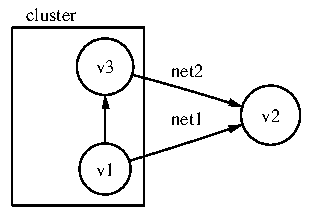
\includegraphics{parallel}
\caption{Parallel edges created during coarsening}
\label{parallel_edges}
\end{figure}


\subsection{Initial Partition Phase}
\label{initial}
This phase is applied to the coarsest hypergraph. Usually initial
partitioning is given by randomly assigning vertices in each partition.
In~\cite{hypergraph_improved_2000}, a new technique was proposed that
initially puts all modules into one partition and then moves a module
only if it does 
not {\it increase the violation} of balance constraints rather than
necessarily result in a legal solution. The method is called VILE
(``Very Illegal'') in~\cite{hypergraph_improved_2000}. 
Observed from our experiments,
the VILE scheme gives significantly smaller final cut-size of the 
benchmark test cases. However, there is a risk that the sequence of
moves may not eventually produce a legal solution. 
Even in the random initialization method, whether the solution is
feasible is not guaranteed when actual area of module is used.
A conservative way is to minimize the different area between two
partitions in this phase. Modules are sorted in
non-increasing order according to their areas
and are put into each partition by the following
rule: always put the next module in the partition of smallest total
area. In gate-level netlist, the number of different areas of modules
is usually small because many modules are in fact from the same master
copy. Thus, we can create a binary search tree for different area type
and ``bucket'' the modules with same area into the same tree node. 
It makes the sorting method take nearly linear time for the flat-FM
algorithm. For the multilevel method, since each 
module/cluster may have different area, the $O(n \log n)$ run time will be
expected.

One problem of our method is that the algorithm is purely
deterministic. In multiple runs meta-heuristic, this will limit the
seach space of our algorithm. We may add some randomness that the
modules with same 
area are inserted to the binary search tree in random order. However,
this only works for the flat-FM algorithm. This raises a question that
which implementation is preferable. Should we choose a more
conservative method or a more aggressive method? In practice, we may
provide two versions of program and let user to choose which version to
use. Finally, a warning message should be displayed whenever the
solution is illegal in both versions.

\subsection{Refinement Phase}
\label{refinement}
Our refinement algorithm is based on the standard Fiduccia-Mattheyses
(FM) heuristic~\cite{FM_1982}. A more detail description is presented
below that follows the reporting method described
in~\cite{hypergraph_reporting_1999}: 

\begin{itemize}
\item 
If two modules from the two gain buckets have the same highest gain and
both of them satisfy the balance constraints, the one which makes better
balance condition will be chosen.
\item
When the delta gain of a move is zero, the gain update will be skipped.
\item
New element in gain bucket will be attached in LIFO fashion.
\item
When selecting the best solution encountered during the pass, the
tie-breaking decision is that the one that makes better balance
condition will be chosen.
\end{itemize}

Note that the nearly linear run-time per pass is expected in this
algorithm if the maximum pin count $p_{max}$ is bounded by a small
value. In gate-level netlist, this assumption is usually
valid. However, in the multilevel method, we may 
create clusters that have high pin counts.
One way to solve this problem may be to switch the conventional priority
queue (which is usually implemented by {\it heap}) whenever $p_{max}$
is large. In our implementation, we simply use the standard FM
algorithm and stop to further generate coarse hypergraphs if $p_{max}$
is detected to be larger than the number of modules.

%% In multi-way partitioning, the implementation is similar to
%% bi-partitioning. we use $k (k - 1)$ gain buckets for updating.
\subsection{Other Implementation Details}
We implemented our algorithms in C++/STL. The source code was compiled
with g++ on a Linux platform.
We use STL data structure for vector, multi-sets, queue, stack, and 
doubly--linked lists. However, the doubly--link lists used in the
bucket structures were implemented in our own code so that they are
fine-tuned for this particular purpose. We use one of the boost
packages for the memory management. The GUI interface was implemented
with Qt package. 


\section{Experimental Results}
\label{experiment}
Our algorithms are tested on a Intel Pentium IV at 1.8GHz PC.
The source code of our algorithms is available upon request.
We use ISPD-98 benchmark Suite
that was downloaded from~\cite{ispd98_benchmark}. The actual area of
module is used in all experiments. All pads are included to be
partitioned. Run-time is measured in second.

\subsection{Comparisons with VILE Initial Partitioning}
Our first experiment compares the performance of our initial partitioning
algorithm described in Section~\ref{initial} with VILE using
our flat-FM code. Table~\ref{vile} reports the minimum cut and the
average CPU time of 100 runs. The balance tolerant $tol$
is set to 2\% of the total area, i.e., [0.49, 0.51]. The actual
different between two partitions (in \%) is given in the third column.

\begin{table}
\renewcommand{\arraystretch}{1.3}
\caption{Comparison of our algorithm and VILE. Average CPU time in
  second is given in parenthesis. Solutions 
  are constrained to be within 2\% of bisection.}
\label{vile}
\centering
\begin{tabular}{|c||c|c|c|c|c|c|}
\hline
 & \multicolumn{3}{c|}{\bfseries Our}
 & \multicolumn{3}{c|}{\bfseries VILE} \\
\cline{2-7}
\bfseries Circuit &  
\bfseries Min  &  \bfseries CPU  &  \bfseries d(\%) &
\bfseries Min  &  \bfseries CPU  &  \bfseries d(\%) \\
\hline\hline
ibm01 &  357 &   0.39 &   0.00 &   226 &   0.23 &   0.64   \\
ibm02 &  363 &   1.09 &   0.26 &   266 &   0.93 &   0.00   \\
ibm03 & 1612 &   1.85 &   0.00 &  1544 &   1.15 &   0.79   \\
ibm04 &  993 &   1.99 &   0.57 &  1397 &   1.07 &   1.88   \\
ibm05 & 2442 &   5.14 &   0.00 &  1864 &   2.80 &   0.00   \\
ibm06 & 1089 &   2.74 &   1.71 &  1017 &   2.19 &   0.00   \\
ibm07 & 1395 &   4.39 &   1.11 &  1325 &   3.88 &   0.63   \\
ibm08 & 1719 &   7.84 &   0.11 &  1624 &   7.83 &   1.10   \\
ibm09 & 2229 &   4.59 &   0.39 &  3017 &   3.50 &   1.51   \\
%% \rlap{\textsuperscript{*}}  \\
ibm10 & 1673 &   7.23 &   0.07 &  1575 &   4.19 &   0.56   \\
ibm11 & 2241 &   6.83 &   1.60 &  3513 &  13.37 &   0.00   \\
ibm12 & 3921 &   9.12 &   0.91 &  2957 &   7.58 &   0.48   \\
ibm13 & 1773 &   8.59 &   0.08 &  1790 &   6.09 &   0.73   \\
ibm14 & 3121 &  38.16 &   0.42 &  3010 &  34.33 &   1.53   \\
ibm15 & 5955 &  22.35 &   1.01 &  5872 &  15.31 &   0.00   \\
ibm16 & 2676 &  31.96 &   0.11 &  3318 &  38.11 &   0.00   \\
ibm17 & 3734 &  52.30 &   0.00 &  4099 &  48.32 &   1.74   \\
ibm18 & 1888 &  55.62 &   1.90 &  2935 &  69.52 &   0.00   \\
\hline
\end{tabular}
\end{table}

At first sight, the VILE scheme produced significant
improvement and all final best solution satisfied the area balance
constraint. But actually within the 100 runs, some of them in fact
could not produce legal solutions, and whenever this happens, the
algorithm stops very quickly and consumes only very small amount of time.

\ 

In the following, we present the
experimental results by using our initial partitioning algorithm only.

%% \subsection{Comparison Single Bucket with Two Buckets}
%% 
%% \begin{table}
%% \renewcommand{\arraystretch}{1.3}
%% \caption{Comparison of single-bucket and two-bucket with actual
%%   area. Solutions are constrained to be within 2\% of bisection.}
%% \label{single_two_bucket_2}
%% \centering
%% \begin{tabular}{|c||c|c|c|c|c|c|}
%% \hline
%%  & \multicolumn{3}{c|}{\bfseries Single Bucket}
%%  & \multicolumn{3}{c|}{\bfseries Two Bucket} \\
%% \cline{2-7}
%% \bfseries Circuit &  
%% \bfseries Min  &  \bfseries CPU  &  \bfseries d(\%) &
%% \bfseries Min  &  \bfseries CPU  &  \bfseries d(\%) \\
%% \hline\hline
%% ibm01 &    284 &   0.43 &   0.03 &    357 &   0.39 &   0.00  \\
%% ibm02 &    375 &   1.10 &   1.59 &    363 &   1.09 &   0.26  \\
%% ibm03 &   1544 &   1.81 &   1.09 &   1612 &   1.85 &   0.00  \\
%% ibm04 &    859 &   1.86 &   1.97 &    993 &   1.99 &   0.57  \\
%% ibm05 &   2497 &   6.48 &   0.45 &   2442 &   5.14 &   0.00  \\
%% ibm06 &    891 &   3.05 &   1.54 &   1089 &   2.74 &   1.71  \\
%% ibm07 &   1477 &   4.45 &   0.00 &   1395 &   4.39 &   1.11  \\
%% ibm08 &   1392 &   8.80 &   1.98 &   1719 &   7.84 &   0.11  \\
%% ibm09 &   1584 &   4.80 &   1.94 &   2229 &   4.59 &   0.39  \\
%% ibm10 &   1998 &   7.81 &   1.37 &   1673 &   7.23 &   0.07  \\
%% ibm11 &   2391 &   6.79 &   1.85 &   2241 &   6.83 &   1.60  \\
%% ibm12 &   3496 &   9.34 &   1.07 &   3921 &   9.12 &   0.91  \\
%% ibm13 &   1693 &   8.11 &   1.47 &   1773 &   8.59 &   0.08  \\
%% ibm14 &   3543 &  46.87 &   1.94 &   3121 &  38.16 &   0.42  \\
%% ibm15 &   5593 &  24.21 &   1.61 &   5955 &  22.35 &   1.01  \\
%% ibm16 &   2469 &  46.43 &   1.94 &   2676 &  31.96 &   0.11  \\
%% ibm17 &   3695 &  65.17 &   0.66 &   3734 &  52.30 &   0.00  \\
%% ibm18 &   2050 &  64.54 &   0.00 &   1888 &  55.62 &   1.90  \\
%% \hline
%% \end{tabular}
%% \end{table}
%% 
%% \begin{table}
%% \renewcommand{\arraystretch}{1.3}
%% \caption{Comparison of single-bucket and two-bucket with actual
%%   area. Solutions are constrained to be within 10\% of bisection.}
%% \label{single_two_bucket_10}
%% \centering
%% \begin{tabular}{|c||c|c|c|c|c|c|}
%% \hline
%%  & \multicolumn{3}{c|}{\bfseries Single Bucket}
%%  & \multicolumn{3}{c|}{\bfseries Two Bucket} \\
%% \cline{2-7}
%% \bfseries Circuit &  
%% \bfseries Min  &  \bfseries CPU  &  \bfseries d(\%) &
%% \bfseries Min  &  \bfseries CPU  &  \bfseries d(\%) \\
%% \hline\hline
%% ibm01 &    325 &   0.56 &   2.81 &    315 &   0.56 &   2.75  \\
%% ibm02 &    349 &   1.08 &   6.15 &    281 &   1.10 &   1.65  \\
%% ibm03 &   1206 &   2.02 &   9.58 &   1309 &   1.75 &   7.29  \\
%% ibm04 &    535 &   2.56 &   9.97 &    726 &   2.79 &   1.70  \\
%% ibm05 &   1999 &   6.85 &   9.95 &   2324 &   5.51 &   0.00  \\
%% ibm06 &    909 &   3.22 &   9.92 &    896 &   3.04 &   9.78  \\
%% ibm07 &    951 &   4.97 &   7.57 &   1083 &   4.49 &   2.90  \\
%% ibm08 &   1460 &  12.00 &   0.39 &   1396 &  11.06 &   0.00  \\
%% ibm09 &    955 &   6.99 &   2.10 &    788 &   5.86 &   0.00  \\
%% ibm10 &   1445 &  12.55 &   9.99 &   1782 &   9.92 &   9.11  \\
%% ibm11 &   1515 &  13.91 &   9.93 &   1757 &   9.36 &   0.00  \\
%% ibm12 &   2486 &  15.78 &   4.19 &   2238 &  13.16 &   9.67  \\
%% ibm13 &   1330 &  10.55 &   9.01 &   1251 &   9.44 &   3.73  \\
%% ibm14 &   1988 &  55.26 &   8.58 &   3013 &  33.73 &   0.00  \\
%% ibm15 &   5052 &  28.37 &   8.44 &   5637 &  23.81 &   4.89  \\
%% ibm16 &   2381 & 113.68 &   8.17 &   2156 &  33.02 &   2.93  \\
%% ibm17 &   3236 & 107.40 &   9.59 &   3340 &  51.09 &   0.00  \\
%% ibm18 &   1999 &  73.20 &   9.59 &   2109 &  56.09 &   0.00  \\
%% \hline
%% \end{tabular}
%% \end{table}

\subsection{Comparison between Various Clustering Approaches}
The comparison of various clustering algorithms is shown in
Table~\ref{clustering_2} and Table~\ref{clustering_10}. 
The partition results are based on the minimum cutsize of 20 runs.
Greedy--MMC refers to the maximal--matching based
clustering with Greedy algorithm. PD--MMC refers to the
maximal--matching based clustering with the Primal-dual algorithm
described in Section~\ref{mmc}. SFC refers to the
signal-flow based clustering described in Section~\ref{sfc}.
We use the cluster size as the net weight in all three methods. In
Table~\ref{clustering_2}, solutions are constrained to be with 2\% of
bisection. In Table~\ref{clustering_10}, solutions are constrained to
be with 10\% of bisection. Average CPU time is given in parenthesis.
Under this framework, PD--MMC outperforms the other two algorithms.

\begin{table}
\renewcommand{\arraystretch}{1.3}
\caption{Comparison of various clustering algorithms in term of
  bi-partitioning results with 20 runs. Solutions are constrained to
  be within 2\% of bisection.} 
\label{clustering_2}
\centering
\begin{tabular}{|c||c|c|c|c|}
\hline
\bfseries ckt & \bfseries size & 
              \bfseries Greedy--MMC & \bfseries PD--MMC & \bfseries SFC  \\
\hline\hline
ibm01 &  12752 &  296 (  0.64) &  274 (  0.51) &  267 (  0.70)  \\
ibm02 &  19601 &  302 (  2.27) &  271 (  1.56) &  319 (  1.66)  \\
ibm03 &  23136 & 1024 (  2.41) & 1138 (  1.78) & 1106 (  2.36)  \\
ibm04 &  27507 &  595 (  2.46) &  537 (  1.87) &  639 (  2.81)  \\
ibm05 &  29347 & 1786 (  3.89) & 1792 (  3.72) & 1765 (  4.00)  \\
ibm06 &  32498 &  807 (  3.91) &  825 (  2.65) &  855 (  3.82)  \\
ibm07 &  45926 &  863 (  4.29) &  937 (  3.92) &  882 (  5.97)  \\
ibm08 &  51309 & 1288 (  7.89) & 1320 (  7.33) & 1391 (  7.97)  \\
ibm09 &  53395 & 1248 (  4.84) &  887 (  4.30) &  809 (  6.24)  \\
ibm10 &  69429 & 1567 ( 13.56) & 1502 (  7.55) & 1518 (  9.96)  \\
ibm11 &  70558 & 1129 (  7.02) & 1134 (  6.65) & 1139 (  8.68)  \\
ibm12 &  71076 & 2363 ( 12.19) & 2361 ( 10.06) & 2521 ( 14.15)  \\
ibm13 &  84199 & 1171 ( 10.14) & 1224 (  8.85) & 1546 ( 13.10)  \\
ibm14 & 147605 & 1995 ( 17.28) & 1966 ( 17.10) & 2070 ( 25.84)  \\
ibm15 & 161570 & 3309 ( 26.29) & 3266 ( 20.06) & 2859 ( 33.93)  \\
ibm16 & 183484 & 1771 ( 25.48) & 1732 ( 22.83) & 1831 ( 34.73)  \\
ibm17 & 185495 & 2668 ( 32.23) & 2542 ( 33.54) & 2583 ( 44.24)  \\
ibm18 & 210613 & 1852 ( 37.33) & 1691 ( 33.91) & 2425 ( 46.54)  \\
%% TOTAL &     -  & 26034 (214.11) & 25399 (188.19) & 26525 (266.72)  \\
\hline
\end{tabular}
\end{table}

\begin{table}
\renewcommand{\arraystretch}{1.3}
\caption{Comparison of various clustering algorithms in term of
  bi-partitioning results with 20 runs.
  Solutions are constrained to be within 10\% of bisection.}
\label{clustering_10}
\centering
\begin{tabular}{|c||c|c|c|c|}
\hline
\bfseries ckt & \bfseries size & 
              \bfseries Greedy--MMC & \bfseries PD--MMC & \bfseries SFC  \\
\hline\hline
ibm01 &  12752 &  260 (0.50) &  217 (0.54) &  219 (0.66)  \\
ibm02 &  19601 &  259 (1.28) &  257 (1.41) &  278 (1.64)  \\
ibm03 &  23136 &  788 (1.53) &  774 (1.57) &  942 (2.11)  \\
ibm04 &  27507 &  447 (1.82) &  481 (1.73) &  445 (2.50)  \\
ibm05 &  29347 & 1734 (3.66) & 1818 (4.09) & 1727 (3.81)  \\
ibm06 &  32498 &  752 (2.37) &  702 (2.43) &  363 (3.42)  \\
ibm07 &  45926 &  770 (3.70) &  740 (3.55) &  761 (4.88)  \\
ibm08 &  51309 & 1154 (6.60) & 1200 (5.95) & 1313 (7.18)  \\
ibm09 &  53395 &  559 (3.72) &  576 (3.54) &  578 (5.24)  \\
ibm10 &  69429 & 1054 (7.69) &  935 (7.60) &  938 (10.07)  \\
ibm11 &  70558 &  781 (5.36) &  730 (5.04) &  757 (7.63)  \\
ibm12 &  71076 & 2129 (9.39) & 2133 (9.25) & 2158 (12.93)  \\
ibm13 &  84199 &  874 (7.66) &  873 (7.62) & 1035 (10.52)  \\
ibm14 & 147605 & 1528 (15.80) & 1580 (15.98) & 1788 (22.43)  \\
ibm15 & 161570 & 2090 (20.66) & 2178 (19.38) & 2288 (26.54)  \\
ibm16 & 183484 & 1779 (22.72) & 1764 (22.50) & 1813 (30.19)  \\
%% \hline
%% TOTAL &     -  & 25058 (205.11) & 25399 (188.60) & 25429 (252.28)  \\
\hline
\end{tabular}
\end{table}

\subsection{Comparison with Other Leading--edge Packages}
We compared two leading--edge multilevel partitioners \verb+hMetis+
(version 1.5.3) and \verb+UCLA MLPart+ (version 4.19) which are
available at~\cite{hMetis} and~\cite{ucla_pdtools} respectively.
First, we use the test case \verb+ibm06+ and set the balance tolerant
to a ridiculously small value 0.001\% such that no feasible solution is
possible. The partitioner \verb+UCLA MLPart+ reported the best
cutsize 4224 as if the solution were legal. This may be explained by
the fact that the VILE initialization scheme is used by the
package. For \verb+hMetis+, since the package only accept the balance
tolerant greater than or equal to 1\%, in order to test if the similar
suitable happen in the hMetis, we modified the area of one module in
the test case to be ridiculously large such that no feasible solution
is possible. Surprisingly \verb+hMetis+ also failed to report any
warning.

%% \begin{table}
%% \renewcommand{\arraystretch}{1.3}
%% \caption{Comparison of our algorithm, UCLA MLPart4.17 and hMetis1.5.3
%%   Solutions are constrained to be within 2\% of bisection. Average CPU
%%   time in seconds is given in parenthesis.}
%% \label{leading_02}
%% \centering
%% \begin{tabular}{|c||c|c|c|c|c|}
%% \hline
%% \bfseries ckt & \bfseries Algo 
%%  & \multicolumn{4}{c|}{2\% configurations} \\
%% \cline{3-6}
%%  ibm\#     &        &    1      &    2      &   3       &    4      \\
%% \hline\hline
%% 01 & hM & 267(5.2)  & 265(7.2)  & 253(11)   & 245(19)   \\
%%    & ML & 250(4.4)  & 238(6.7)  & 231(11)   & 227(20)   \\
%% 02 & hM & 320(10)   & 314(14)   & 302(20)   & 299(33)   \\
%%    & ML & 348(8.0)  & 335(12)   & 313(22)   & 294(40)   \\
%% 03 & hM & 885(16)   & 869(20)   & 859(28)   & 855(45)   \\
%%    & ML & 903(10)   & 883(15)   & 847(27)   & 818(48)   \\ 
%% 04 & hM & 550(13)   & 543(18)   & 535(28)   & 534(45)   \\ 
%%    & ML & 592(12)   & 575(18)   & 546(34)   & 531(60)   \\ 
%% 05 & hM & 1777(22)  & 1749(27)  & 1744(41)  & 1741(69)  \\ 
%%    & ML & 1841(17)  & 1810(26)  & 1759(44)  & 1750(79)  \\
%% 06 & hM & 728(24)   & 679(30)   & 637(41)   & 605(65)   \\
%%    & ML & 696(14)   & 664(22)   & 633(37)   & 564(65)   \\
%% 07 & hM & 855(42.2) & 859(54.5) & 824(63.5) & 794(101)  \\ 
%%    & ML & 846(20)   & 840(31)   & 812(53)   & 793(94)   \\ 
%% 08 & hM & 1246(52)  & 1216(57)  & 1211(74)  & 1208(130) \\
%%    & ML & 1354(25)  & 1342(39)  & 1238(65)  & 1206(112) \\ 
%% 09 & hM & 591(33)   & 530(42)   & 527(62)   & 524(98)   \\ 
%%    & ML & 555(22)   & 534(35)   & 528(56)   & 527(91)   \\ 
%% 10 & hM & 1310(78)  & 1273(97)  & 1215(126) & 1193(192) \\ 
%%    & ML & 1419(33)  & 1397(53)  & 1322(90)  & 1211(157) \\ 
%% 11 & hM & 914(67)   & 883(77)   & 845(100)  & 813(150)  \\
%%    & ML & 926(32)   & 908(50)   & 862(79)   & 842(136)  \\ 
%% 12 & hM & 2304(99)  & 2180(126) & 2150(154) & 2131(241) \\ 
%%    & ML & 2676(32)  & 2578(55)  & 2498(88)  & 2353(153) \\
%% 13 & hM & 1110(103) & 1009(107) & 956(134)  & 931(208)  \\ 
%%    & ML & 1247(41)  & 1200(63)  & 1140(103) & 1036(180) \\ 
%% 14 & hM & 2092(211) & 1992(258) & 1910(369) & 1865(607) \\
%%    & ML & 2043(80)  & 2035(121) & 1917(205) & 1860(316) \\
%% 15 & hM & 2435(270) & 2418(323) & 2366(399) & 2221(597) \\ 
%%    & ML & 2486(85)  & 2464(138) & 2378(225) & 2243(397) \\ 
%% 16 & hM & 2165(292) & 1829(327) & 1732(451) & 1713(695) \\
%%    & ML & 2040(104) & 1983(163) & 1869(263) & 1853(455) \\
%% 17 & hM & 2610(426) & 2521(471) & 2491(645) & 2460(996) \\
%%    & ML & 2437(113) & 2413(173) & 2382(303) & 2353(544) \\
%% 18 & hM & 1833(334) & 1836(439) & 1754(640) & 1706(1064)\\ 
%%    & ML & 2002(128) & 1976(190) & 1823(399) & 1737(612) \\
%% \hline
%% \end{tabular}
%% \end{table}
%% 
%% \begin{table}
%% \renewcommand{\arraystretch}{1.3}
%% \caption{Comparison of our algorithm, UCLA MLPart4.17 and hMetis1.5.3
%%   Solutions are constrained to be within 10\% of bisection. Average CPU
%%   time in seconds is given in parenthesis.}
%% \label{leading_10}
%% \centering
%% \begin{tabular}{|c||c|c|c|c|c|}
%% \hline
%% \bfseries ckt & \bfseries Algo 
%%  & \multicolumn{4}{c|}{10\% configurations} \\
%% \cline{3-6}
%%  ibm\#     &        &    1      &    2      &   3       &   4       \\
%% \hline\hline
%% 01 & hM & 255(5.3)  & 252(7.3)  & 247(11)   & 237(18)   \\ 
%%    & ML & 238(4.6)  & 233(6.9)  & 223(12)   & 220(21)   \\ 
%% 02 & hM & 279(11)   & 279(14)   & 279(19)   & 278(31)   \\ 
%%    & ML & 291(8.2)  & 291(13)   & 272(21)   & 268(37)   \\ 
%% 03 & hM & 779(15)   & 776(18)   & 768(27)   & 759(43)   \\ 
%%    & ML & 802(11)   & 783(16)   & 732(30)   & 705(52)   \\ 
%% 04 & hM & 506(19)   & 510(20)   & 492(29)   & 478(51)   \\ 
%%    & ML & 535(12)   & 512(19)   & 482(32)   & 468(56)   \\ 
%% 05 & hM & 1759(25)  & 1740(28)  & 1731(42)  & 1725(67)  \\ 
%%    & ML & 1773(17)  & 1726(26)  & 1728(43)  & 1716(77)  \\ 
%% 06 & hM & 402(24)   & 383(26)   & 374(35)   & 370(55)   \\ 
%%    & ML & 465(14)   & 433(22)   & 394(34)   & 375(61)   \\ 
%% 07 & hM & 809(40)   & 806(46)   & 796(63)   & 764(102)  \\ 
%%    & ML & 790(20)   & 786(32)   & 760(52)   & 747(93)   \\ 
%% 08 & hM & 1166(43)  & 1162(51)  & 1161(75)  & 1159(123) \\ 
%%    & ML & 1348(25)  & 1330(40)  & 1195(66)  & 1168(113) \\ 
%% 09 & hM & 664(33)   & 540(42)   & 528(59)   & 525(96)   \\ 
%%    & ML & 572(21)   & 560(34)   & 556(55)   & 527(90)   \\ 
%% 10 & hM & 842(57)   & 830(72)   & 798(102)  & 779(169)  \\ 
%%    & ML & 1196(35)  & 1132(55)  & 1023(91)  & 938(161)  \\ 
%% 11 & hM & 828(59)   & 744(71)   & 717(103)  & 710(155)  \\ 
%%    & ML & 788(30)   & 779(48)   & 745(77)   & 728(124)  \\ 
%% 12 & hM & 2326(83)  & 2165(108) & 2135(153) & 2047(238) \\ 
%%    & ML & 2349(38)  & 2304(57)  & 2261(102) & 2206(176) \\ 
%% 13 & hM & 1045(97)  & 999(104)  & 940(129)  & 902(197)  \\ 
%%    & ML & 1095(38)  & 1058(61)  & 1027(99)  & 963(176)  \\ 
%% 14 & hM & 1894(212) & 1776(250) & 1682(351) & 1599(565) \\ 
%%    & ML & 1759(67)  & 1727(104) & 1638(167) & 1590(300) \\ 
%% 15 & hM & 2073(264) & 2032(301) & 1910(402) & 1866(564) \\ 
%%    & ML & 2244(83)  & 2029(133) & 2035(221) & 1975(385) \\ 
%% 16 & hM & 1942(232) & 1754(311) & 1829(327) & 1721(709) \\ 
%%    & ML & 1976(102) & 1915(155) & 1752(257) & 1714(460) \\ 
%% 17 & hM & 2417(408) & 2372(467) & 2337(635) & 2311(987) \\ 
%%    & ML & 2316(105) & 2294(170) & 2264(290) & 2239(385) \\ 
%% 18 & hM & 1632(306) & 1617(357) & 1561(601) & 1536(836) \\ 
%%    & ML & 1976(104) & 1955(160) & 1666(365) & 1595(612) \\
%% \hline
%% \end{tabular}
%% \end{table}

\verb+hMetis+ provides serveral different coarsening schemes, uncoarsening
schemes and V-cycle refinement schemes. We use the \verb+shmetis+
in which the default schemes are set. Table~\ref{leading_10} presents
bi-partitioning results for actual area and allowing up to 10\%
derviation from exact bisection. We use the Primal-dual clustering
algorithm for our implementation in this experiment. Cluster size
is used as the net weight in the Primal-dual algorithm. The initial
paritioning solution of the coarsest hypergraph is obtained from the
best of three runs of the FM algorithm. The best solution of three
runs of our multilevel method is reported and the total CPU time is
given in parenthesis. The result shows that our multilevel method
produces very promising quality of solution even thought both aggressive
strategies and non-trivial fine-tuning techniques have not been used.

\begin{table}
\renewcommand{\arraystretch}{1.3}
\caption{Comparison of hMetis1.5.3, UCLA MLPart4.19 and our algorithm.
  Solutions are constrained to be within 10\% of bisection. Average CPU
  time in seconds is given in parenthesis.}
\label{leading_10}
\centering
\begin{tabular}{|c||c|c|c|}
\hline
\bfseries ckt & \bfseries shmetis & \bfseries UCLA ML & \bfseries OUR \\
\hline\hline
ibm01 & 248(4.04)   & 240(1.19)   &  217(1.71)    \\
ibm02 & 284(6.15)   & 310(2.45)   &  258(4.57)	  \\
ibm03 & 805(8.87)   & 722(3.09)   &  1143(5.67)	  \\
ibm04 & 445(10.61)  & 477(3.07)   &  502(5.29)	  \\
ibm05 & 1725(16.41) & 1741(6.39)  &  1805(13.88)  \\
ibm06 & 368(15.90)  & 484(4.66)   &  777(8.28)	  \\
ibm07 & 749(27.78)  & 775(6.56)   &  778(12.37)	  \\
ibm08 & 1159(33.42) & 1225(8.27)  &  1215(20.16)  \\
ibm09 & 522(25.57)  & 520(8.27)   &  606(12.25)	  \\
ibm10 & 769(47.06)  & 871(12.56)  &  1011(23.03)  \\
ibm11 & 737(42.43)  & 745(11.80)  &  737(16.66)	  \\
ibm12 & 1976(62.48) & 2741(14.57) &  2152(24.48)  \\
ibm13 & 876(46.53)  & 1121(15.69) &  912(23.16)	  \\
ibm14 & 1578(153.6) & 1875(30.71) &  1665(50.70)  \\
ibm15 & 1939(171.7) & 1947(40.31) &  2498(58.46)  \\
ibm16 & 1716(212.7) & 1684(45.55) &  1750(61.97)  \\
ibm17 & 2249(280.6) & 2291(56.69) &  2420(102.72) \\
ibm18 & 1539(227.0) & 2042(53.39) &  1864(82.77)  \\
\hline
\end{tabular}
\end{table}

\section{Conclusion}
\label{conclusion}
We have presented two new clustering algorithms, namely the
Primal-dual algorithm and the Signal-flow based algorithm. The Primal-dual
algorithm outperforms the greedy algorithm which is
commonly used in the circuit partitioning literature. 
The signal-flow based algorithm does
not seem to be efficient for this area-constrained net-based problem.
However, we believe that the algorithms developed in this paper are
useful for the path-based problem and the performance-driven problem.

\section*{Acknowledgment}
The author would like to thank...~\cite{ispd98_benchmark}

%\bibliographystyle{abbrv}
\bibliographystyle{IEEEtran.bst}
\bibliography{IEEEabrv,part}

\end{document}
